%!TEX root = project.tex

\chapter*{Abstract}
\paragraph{Abstract}
For my final year project, I was looking to create a project that would offer the chance for users to bet and lay on sporting events. A betting exchange is something I have become very interested in recent times and thought that this would be a great opportunity to research the subject and develop my own solution. I wanted to develop this as a web application where a user can create an account, top-up their account, place bets and also lay bets. The bets are populated and set via pulling data from other popular betting companies to get the best price possible. I created this application with a client and server pulling data from the data from the databases. It is a three-tier architecture application using a MySQL data base in the data tier, PHP on the logic tier and HTML and BootStrap for the Presentation tier.

\paragraph{Authors}
Colm Woodlock



\chapter{Introduction}
When choosing my project, I wanted to pick something that was relevant to what I was interested in and something that I might find useful. This project would also have to highlight my existing skills but also offered some space to learn new skills and research a topic I may not be fully familiar with. With this criteria in mind I started to brain storm ideas on some of the things that I might like to do. 

In the end I settled on a web application called BetEx. BetEx would be a betting exchange. My reason for choosing this is as a few years ago like many other college student was looking for some way to make some extra money on the side with as little effort as possible. That is when I stumbled across a site called OddsMonkey~\cite{oddsMonkey}, on this site they claimed if you followed their guides and tips a user could claim free money that bookmakers were simply giving away. Having seen the offers for "Bet €20 get €20" all over television advertisements, billboards, newspapers and websites, I always thought to myself there must be a way of taking advantage of this but never gave it much more thought. Upon reading their guide I gave it a go and low and behold I had turned my free €20 bet into €15 of take home money with minimal effort. From there I did more research discovering new methods, all the while reaping the benefits of them. This has funded both my education and various holidays. A key component to matched betting is the betting exchange and not many exist on a large scale BetFair, Smarkets and Matchbook being the largest of them~\cite{companies}. This lead me to the idea to develop my own platform to try and understand the workings behind the scenes of a betting exchange. I felt like there was an opportunity to make an exchange that had a much more user friendly interface as I found working with some of the established companies websites to be very confusing at the start.
Once the project idea was decided on I then had to think about what technologies I wanted to use. I wanted to use many different types of technologies in order to demonstrate my ability but also some that I would have to learn to show my capability to learn new things and incorporate them into an application. In the end I settled on a three tier structure containing a HTML and Boostrap presentation tier, a PHP logic tier which would offer new learning experiences and also for the data tier I would be using a MySQL database.
From all of this I hoped that I would achieve a product in the end that would meet my expectation of both myself and the expectations worthy of a final year project in a Software Development course.

\chapter{Context}
The context of my application is to offer a service to users who are new to laying bets. On the site a user can create an account, top-up their account and place a bet/lay from a list of real and regularly updated events.
\begin{itemize}
\item Log-in.
\item Top-up.
\item Place bet/lay.
\end{itemize}

\section{Objectives}
\subsection{Home Page}
The objective of the home page is to offer a landing platform for the user. Here they will be presented with the navigation for the website such as access to log in and register pages. A user who is not logged in may not have access to some other features presented on the home page.

\subsection{Register Page}
The register page offers a form to the user where they can securely create an account for the web application. Once the form is filled out correctly and successfully the user automatically sent out an email for confirmation.

\subsection{Log in Page}
The log in page allows users who have already registered for the site to access their account. Here they enter their email and their password which is stored as a hashed value. The logic behind the page then compares the password entered to the hashed value that is stored in the database. If the passwords match the user is logged in and they now have access to more features.

\subsection{Activation Page}
The activation page is used for when the user registering. A code will be automatically generated and emailed to the user to their provided email account and once entered the user will then be fully registered.

\subsection{Forgot Password Page}
Similar to the Activation page the user will be sent a code that is automatically generated and emailed to their provided email account. Once the user enters this code and it is correct they will then have the opportunity to change their password.

\subsection{Top up Page}
Provided the user is logged in they will have access to the top-up page. Here the user will be able to enter their details and the top-up amount will be added to their account to be used when betting/ laying on events.

\subsection{User Page}
The user page will be available once the user is logged in, here it will display information that is personal to that user such as their active bets or their account credits.

\subsection{Available Bets Page}
On the available bets page the user will be able to see the events that are currently available to bet/lay on. 

\subsection{Bet/Lay Page}
On this page, once the user has selected an event to bet on they will be given the opportunity to select an amount they wish to place a bet/lay on the event. Once it is placed it will be assigned to their account which they will be able to see on their user page.

\section{Project Links}
The full project is available here on GitHub:
https://github.com/cwoodlock/4thYearSoftwareProject

\section{Chapter Review}
This paper is broken down into various chapters ranging from the planning of the project to the design and implementation of a solution. The following sub-sections will give you a brief overview of each chapter in the paper.

\subsection{Methodology}
In this chapter I will discuss some of the methodologies I used during the various stages of creating the betting exchange web application. In this section I discuss Agile, version control, testing and sprints.

\subsection{Technology Review}
In the technology review chapter I review the various technologies that I used in the development of my project. I review everything from the back and front end technologies to development tools and version control.

\subsection{System Design}
In this chapter I give an explanation of the overall architecture of the betting exchange. I explain why I decided to do certain things and how I implemented those decisions into the project.
\subsection{System Evaluation}
In this chapter I evaluate the system in regards to robustness, testing, test results and limitations. 

\subsection{Conclusion}
Finally in the conclusion I summaries the project against what I set out to do in the goals and objectives. I review the application from the various stages of development and I talk about the possible future developments with the project.

\chapter{Methodology}
In this chapter i will discuss the methodologies used in this project. A methodology is just a way to plan and control the development process of a piece of software effectively. There are many different types of methodologies such as extreme programming or waterfall but for this project I tried to used Agile as my main methodology.

\section{Agile Development}
During the life cycle of this project I attempted to use agile as my main methodology whenever I could. I used this approach during all stages which included the research, design and implementation. In the initial stages of the project I was considering what methodology to use but ultimately decided on using agile as it is what is used by a lot of companies at the moment and I was interested in trying to replicate their approach to developing software.

There are different styles of agile development such as KanBan or extreme programming, but the one I chose for my approach to the project was scrum. Scrum is an agile methodology in which a cycle is carried out in what are known as sprints. 

Throughout the life cycle of the project I held weekly meetings with my project advisor. In these meetings we would discuss what I had done in the previous week and what I was planning to achieve in the following week. Whatever was decided at these meetings, I then created cards on the GitHub project board on the projects page. This helped me focus on the task at hand and I found using this project board to be very useful in the development of this project. Once I started the particular task I would edit the project board and move the card to the in progress column and upon completion of the task move it to the completed section.  

\section{Version Control}
Throughout the life cycle of the project I used GitHub for the version control. GitHub is a hosting service for version control. What I did was created a repository on GitHub and during the development of the project I would commit whatever progress I had made during that session to GitHub to record my progress. 

Tracking the source code I was committing to GitHub was not the only service I used, I also used the task management tool. This allowed me to create tasks that I wanted to complete and assign them to various sections such as to-do or in progress. 

GitHub also provided an opportunity for me to share my work with my project advisor in weeks I could not attend the project meeting. On the repository you can see when new things are committed and what exactly was updated. Another feature I used with GitHub was the ability to rollback the project if needed. Github Tracked the entire progress of the project and at any time I could revert back to any of the previous commits and this proved very useful.

\section{Testing}
For my application I needed to decide how I was going to test the application as I could not use something such as J-unit. In the end I decided to go with white and black box testing. We had looked at this method of testing in a previous module and I thought it was fit the purposes  of testing that I needed.

\subsection{White Box Testing}
In white box testing the tester can see in internal workings of the software. White box testers have a full and comprehensive knowledge of the internal makeup of the software and are usually software developers themselves. This is a role I thought I suited and so I carried out the software tests. What I did was I wrote out some features I would like to test and the expected outcome. For example if I was testing the log-in system, the expected outcome would be that the user is logged in and is presented their user page. I would then test this and follow the path the program follows as it moves down through the code.

\subsection{Black Box Testing}
Black box testing is a way of testing a piece of software without knowing the internal functionality of the software being tested. A black box tester has no knowledge of the internal design, structure or implementation of the software and are often not software developers. For this I asked some of my friends to test out certain features of the software. The web application was hosted on the Google cloud platform and so I was able to send them a link and ask them to try and perform certain functions. Again I would have made a list of expected outcomes and asked them to recommend any changes if they found any problems themselves. I found this very useful as I often skipped over something small from being so used to looking at it the whole time.

\section{Sprints}
In this section I will be talking about sprints. Each of the sprints I tried to complete in a timely manner and as effectively as possible. Each sprint represents a vital part of the application.

\subsection{Sprint 1 Research}
This was my first sprint and I used it to research existing exchanges. I focused on understanding what was user-friendly and how I could potentially improve on existing solutions.

\subsection{Sprint 2 Design}
During this sprint I focused on the design of the application. Not the aesthetic design but rather the database structure and web application structure.

\subsection{Sprint 3 Database Connection}
Once the design was complete it was time to start the first of the implementation sprints. For this sprint the objective was to set up a basic three-tier solution. For this I stored some data in a database and using php I presented it on a web page. 

\subsection{Sprint 4 Log-in and Registration}
Once the basic pipeline was implemented I then decided to work on a log-in system. This log-in system would be pretty comprehensive in regards to the validation checks, cleaning the data before storage in the database and creating a unique session for each user. 

\subsection{Sprint 5 Website Design}
Once the log in system and registration system was implemented I then decided to work on the general website design. I created a home page where a user could log in from and a user page available only to the logged in user and also general website navigation.

\subsection{Sprint 6 User Validation}
This was the sprint where I finished off the user validation I added a system to email the user an activation code when registering and also an activation code when trying to reset passwords. All of these help with the security of the site.

\subsection{Sprint 7 Sessions}
During this Sprint another feature I added in this, was the remember me function. This used session data to remember the user from a particular session and not require the user to log in providing the session has not ended.
 
\subsection{Sprint 8 Top up account}
During this sprint I wanted to add functionality to the user to be able to top up their account have have credit to use on betting/laying events.

\subsection{Sprint 9 Display Data from Database}
This was a very important sprint as it was the one where I pulled the data on the events and presented them to the user so that they could then place a bet or lay on the event.

\subsection{Sprint 10 Place a Bet/Lay}
Now that the data was being displayed, during this sprint I allowed the user to place bets or lays on their selected event. This bet/lay would then be assigned to their account so that the user could see what bets/lays they have placed.

\subsection{Sprint 11 Python Scraper}
The final sprint was to implement a python scraper that would be used to populate the database for the events. This script would be running on the web server and continually updating the data that was being presented to the user.

\chapter{Technology Review}
In this section, I will cover the overall design and architecture of the application. I will do this through using code snippets to help to understand the design. The technology review chapter will be broken up into three sub sections which will be the data tier, logic tier and presentation tier. An aditional subsection will be used for other technology I used that may not fit into the 3 tier structure.

\section{Data Tier}
The data tier represents the overall stored data and gives the ability to store, access, update and delete certain data. For my application I have only one database. This database is used to store user information, events and betting/laying information.

\subsection{MySQL}
I chose MySQL to handle all of my database needs as I have used it before and I think it works very easily with php. There are some issue with using MySQL such as sql-injection but I have made some simple functions to mitigate this in my application. In this database I am storing table which will contain all the user, event and placed bets data. During the making of the application these tables and the structure of the database changed many times using a MySQL database with phpMyAdmin made it very easy to change and rearrange the database when needed.

As of writing this dissertation I do not have it implemented but the original plan was to get a working web scraper in python and scrape data into a database. Scraping data to a sql file isn't too challenging and this was another reason that I chose to use a MySQL database. Overall it fulfilled my needs and the needs of the application. 

\section{Logic Tier}
\subsection{Php}
PHP is a general-purpose programming language originally designed for web development in 1994 by Rasmus Lerdorf~\cite{php} . There are a few reasons I chose to use PHP in my project over more modern and appealing node js and go, one of these reasons was we covered javascript and go on this course in some modules and I wanted to show my ability to learn something different that we havn't been though on this course. Another reason being is that I had some experience with PHP before on a a previous project I did and I enjoyed PHP development. So with these in mind I thought it suited what I wanted to achieve in this application.

\subsection{Python}
Python is a programming language that is very interesting and very powerful. Having had some experience with Python throughout the course I wanted to incorporate it somehow into my project. The plan was to use the many API's available within python to scrape data from a website then use it to create a sql database of information that would be continually updated. As I have mentioned before I have not implemented this into the project in the time of writing this but I hope to have it implemented in the live project, available on GitHub.


\section{Presentation Tier}
\subsection{HTML}
HTML5 or Hypertext Markup Language is a standard markup language for creating web pages and web applications. Using it in conjunction with PHP was an integral part of my project. Using it allowed me to prototype pages quickly to check interactions and functions I had written in PHP. Once the page demonstrated that it was functioning correctly it was very simple to implement Bootstrap into the pages to make them appear more aesthetically pleasing.

\subsection{jQuery}
jQuery is a javascript library. Using this allowed me to add animations to certain interactions. Combined with the styling from Bootstrap some of this animations made the functionality of the web application not only interactive but also aesthetically appealing.

\section{Additional}
\subsection{CSS}
I used CSS or Cascading Style Sheets in a number of places in this project. CSS allows the user to style their web page from the standard HTML page. This adds uniqueness to the application and also appeals to the eye. The main place I used this was in editing the existing Bootstrap.css file that is provided when using Bootstrap. I edited it to provide a custom Bootstrap theme that would be unique to my web application.

\subsection{Bootstrap}
There are many reasons to use Bootstrap and having used it before it was an easy decision for me ti include it in my project. Bootstrap is a framework for HTML, CSS and JS for responsive development.  One of the main reasons I decided on using it is that it saves time when you are designing your web pages. It is very easy to use templates and classes and simply plug them into your application and in most cases this will work almost immediately. Another reason I decided to used Bootstrap was that it is very easy to customise. Making this themes unique and personal to me is very easy to do and this was again another factor into why I chose to use Bootstrap. The is also extensive documentation that comes with Bootstrap, providing live examples and all the various options available to the user, this makes it very easy to decide on what you want to implement into your web application and then do it. 

\subsection{LaTeX}
LaTex is a typing system that is used throughout industries. It works on a scripting programming language. LaTex is not as simple and as user friendly as something such as Microsoft Office or Google docs however it is a much more powerful tool in regards to customisation and referencing in particular. I have used LaTex in previous modules and has since become my regular document writing application. For instance this dissertation is being written in LaTex. It can be quite difficult to understand in the beginning however with some practise and understanding of some of the easier commands you quickly get the hang of it. Another feature from LaTex is the ability to control the layout of the file, using simple commands a user can change the appearance of a file very easily.

\section{Technologies Used}
\subsection{Sublime Text}
As I was developing the majority of my project in PHP I did not require a large IDE such as Microsoft Visual Studio, instead I could use a simple light weight editor. I searched for some alternatives and found Sublime Text was the application that suited my goals best. It allowed for easy project management, readable colour scheme for php and also git integration that allowed for quick and easy commits to GitHub. Overall I have no complaints about Sublime Text and it accomodated everything that I asked for it in regards to the web application that I made. 

\subsection{phpMyAdmin}
phpMyAdmin was used to manage the databases I was using throughout the development of the project. Having used it before it was very easy to view and manage databases. The UI may be slightly confusing to users who are not familiar with the layout however it doesn't take long to get used to it and navigate the application with ease.

\subsection{GitHub}
GitHub is a hosting service and it allows users to hose, shar and collaborate on projects together. It is often used in open source projects. Projects hosted on GitHub are called repositories and it is here that a user can save their projects to, pull down changes that a collaborator has made or push up changes they have made themselves. It is a very powerful tool and one I have become used to using with all of my projects.

Despite not collaboration with anyone on this project Github still proved a valuable tool. One of the reasons it proved a valuable tool was that it allowed me to track my progress and also allowed me to share my progress with my project advisor though out the life cycle of the project. 

\subsection{Google Cloud Services}
Google Cloud Service provided a a quick and easy solution to host a live version of my web app. Having installed wamp onto the virtual machine it was very simple to configure and display a static version of my web application at a certain ip address.

\subsection{WAMP}
WAMP stands for Windows Apache MySQL PHP and it is a package used by PHP developers to develop web apps. This was the perfect too for me as it comes installed with Apache server , MySQL database , phpMyAdmin and PHP all things I had identified that I wanted to use in my project. having used it before as part of a module it proved an ideal candidate to include into my project and worked without any issues.

\subsection{Overleaf}
Overleaf is an online real time editor used for editing LaTex. This means that I did not have to install specialist software in order to edit the LaTex files that I would be using to write my dissertation for this project. I had used it before in another module and was familiar with the user interface.

Overleaf offers a lot of features that was suitable for my project. I could share my pr ogres with my project advisor and it also offers the opportunity to link the files directly to your GitHub repository.

\subsection{Cmder}
Commander is a console emulator for Windows that allows the user to use some Linux commands on a windows machine. I mainly used this for merge conflicts and other issues I was having with GitHub when pulling or pushing commits. This wasn't too often but it was a tool that I found very useful and worth mentioning in this project.

\chapter{System Design}
In this dection, I will be going over the overall design and architecture of the application. I will go though some code snippets that I will use as a visual aid to help you get a better understanding of what is going on in the application. I have broken down this section into 3 parts, the data tier, logic tier and the presentation tier. 

\section{Data Tier}
The data tier represents the overall stored data in the application and gives the user the ability to store, read, update and delete the data contained within. I have a single database that is used to store the users, the events and also the bet information. The figure below shows the structure of the database.

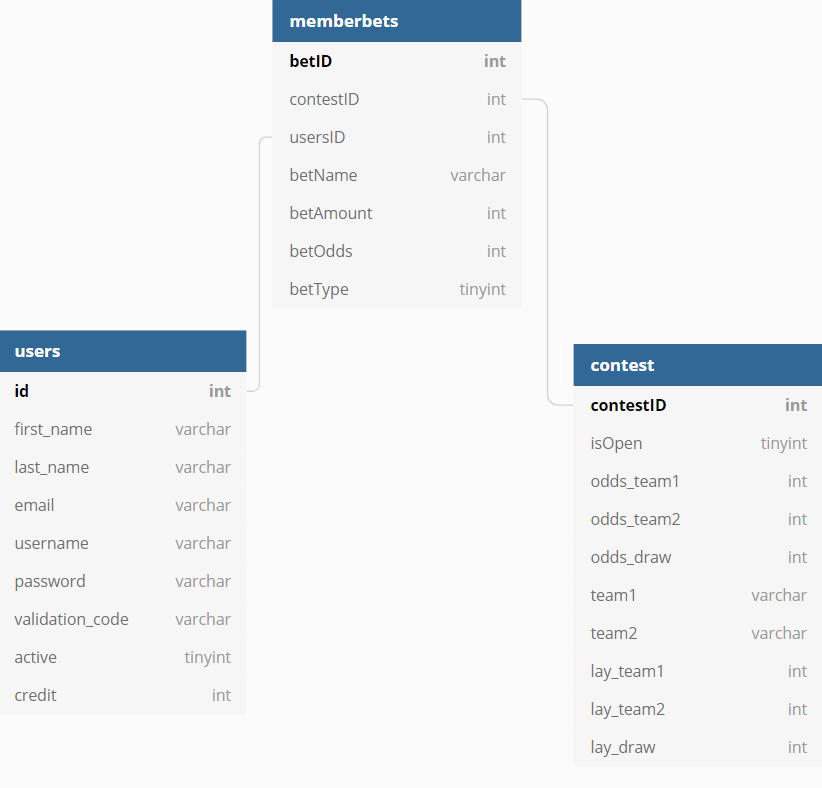
\includegraphics[width=6cm, height=6cm]{img/DatabaseFinal.png}


\subsection{MySQL}
I chose MySQL to handle off the database requirements of the application as I was familiar with it and there are many resources online. I wanted to create a log in system that allowed a user to register, log in if they already have an account, account verification, forgotten password functionality and remember me functionality. 

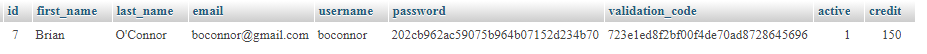
\includegraphics[width=\textwidth,height=\textheight,keepaspectratio]{img/Users.png}

In the image above you can see I am storing the password and validation code as hashed values.
This is achieved in the functions during the registration phase.

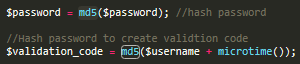
\includegraphics[width=\textwidth,height=\textheight,keepaspectratio]{img/hash.png}

Overall phpMyAdmin in conjunction with the mySQL database I created was very easy to work with and provided all the functionality I wanted to implement.

\section{Logic Tier}
The logic tier refers to the logic behind your application. This is where the majority of the data manipulation is done. This can include creation of new data, storing data, updating and deleting data. To handle this logic I decided to use PHP. It was very easy to integrate the database into the php logic. 

The first thing I wanted to establish in the data tier was a solid connection that i could all on each time I wanted to access the database, I also wanted a few key functions that I would use repeatedly throughout the project. Below is an image of these functions which I placed in their own php file called db. This php file would be included in every php file I wrote after this.

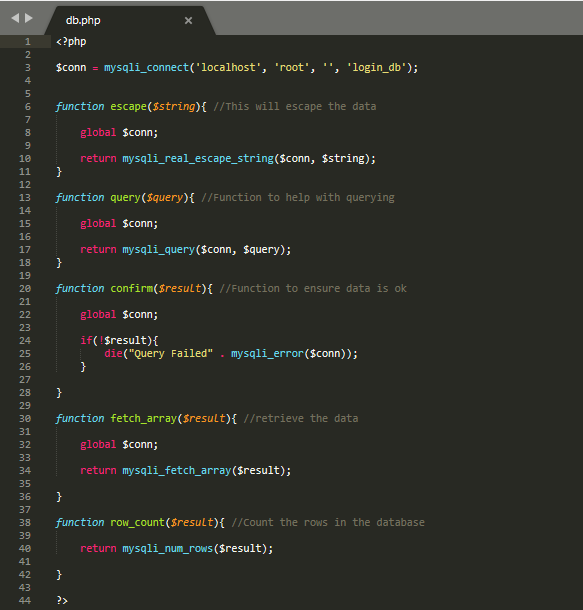
\includegraphics[width=\textwidth,height=\textheight,keepaspectratio]{img/db.png}

Most of these functions are pretty standard and are just ways to access existing functions easier however one I would like to highlight is the escape function. This is used to sanitise the data that is being passed into it this is to help minimise the risk of sql injection which is a common problem with a sql database.

The next thing that I felt was appropriate to implement was the log in system. The logic being this was simple enough as it has been done many times over and so I has able to use these examples as reference for my system. To create the register system there were some functions I thought were important to include was a check to see if the user name exists already in the database and also if the email already exists. Below is the code that I used to complete these checks.

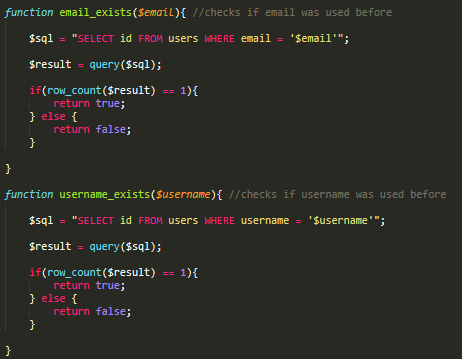
\includegraphics[width=\textwidth,height=\textheight,keepaspectratio]{img/emain-user-check.png}

Next I had to implement these checks into a validation system. This was my second layer of validation as there was some validation check already happening with HTML5.

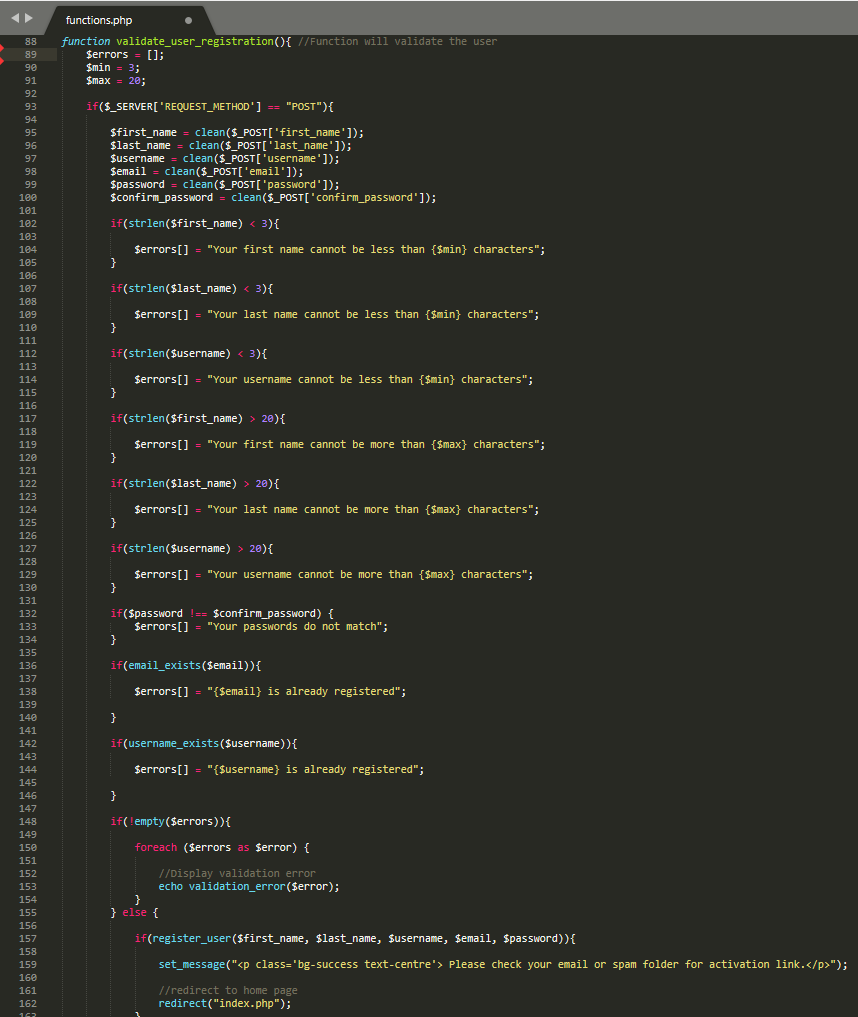
\includegraphics[width=\textwidth,height=\textheight,keepaspectratio]{img/validationRegister.png}

Providing the user had passed all these checks the information would then be passed into the registeruser function where the users information would be stored in the database and a validation code would be generated which would then be sent out to the user via email. It is worth noting that this function does not work on localhost unless you configure the localhost to do so.

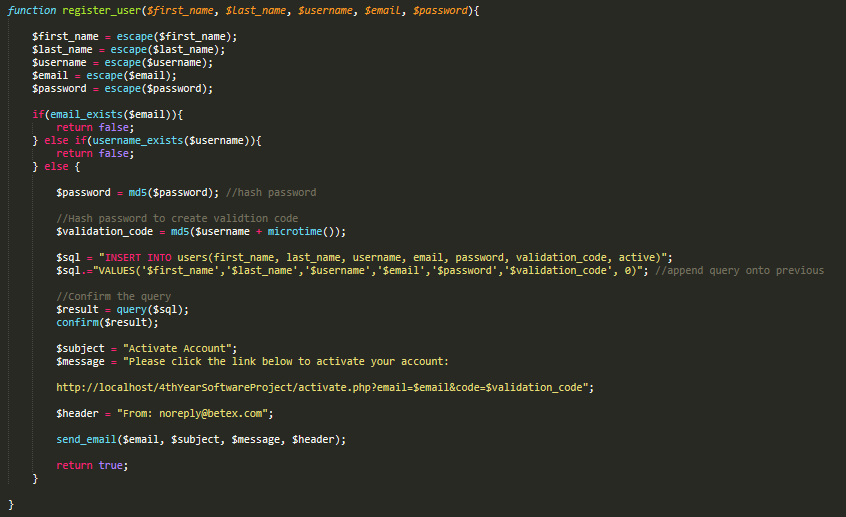
\includegraphics[width=\textwidth,height=\textheight,keepaspectratio]{img/register.png}

At this point the account is created however the account must be activated in order to use it. If an email is sent out the user can click the link and they will be sent to an activation page on the site where they can enter the validation code that was also sent out in the email. Below is the code that is used to activate the account of the user.

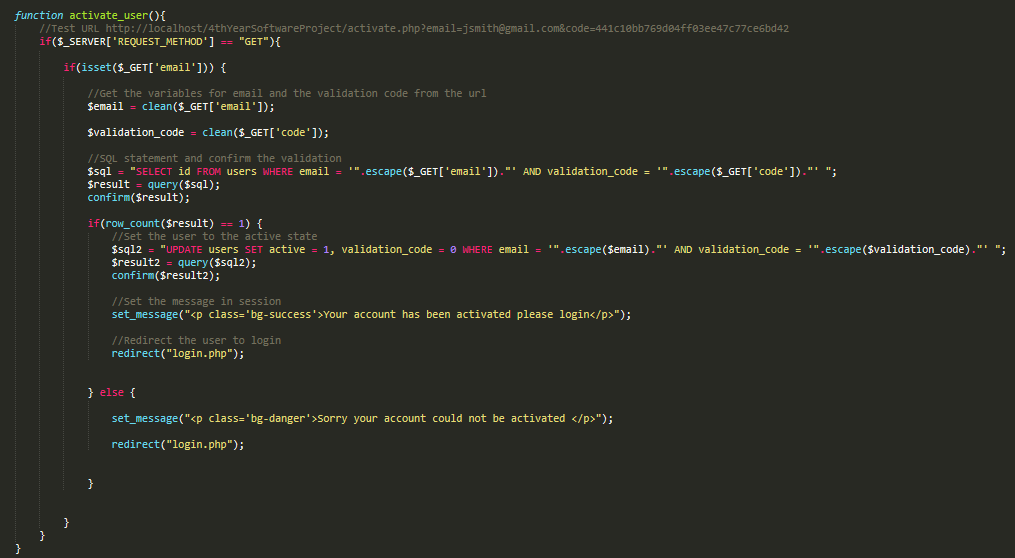
\includegraphics[width=\textwidth,height=\textheight,keepaspectratio]{img/activate.png}

Now the user has a fully activated account and can now log in. Much like the register system the log in system must have similar validation. This is to ensure the correct data is being entered and no input fields are being left blank or contain invalid data.

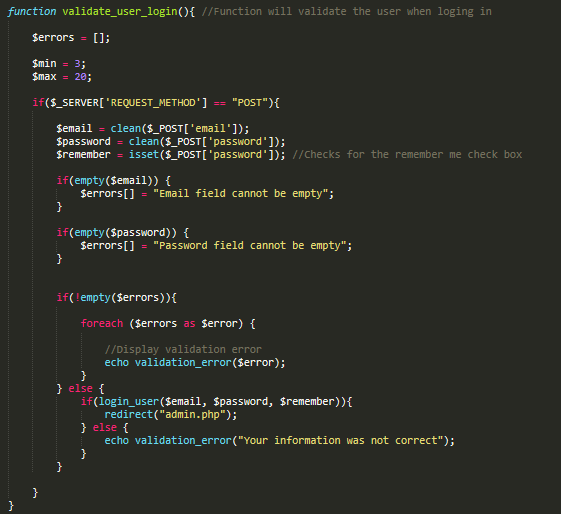
\includegraphics[width=\textwidth,height=\textheight,keepaspectratio]{img/validateLogin.png}

Again once the user passes the validation their information is passed into a log in function to log the user in. In this function the hashed password is retrieved from the database and compared to the hashed version of the entered password. If there is a match I the application then starts a session and saves the logged in email into the session. This will be used at a later time when we discuss the remember me functionality.

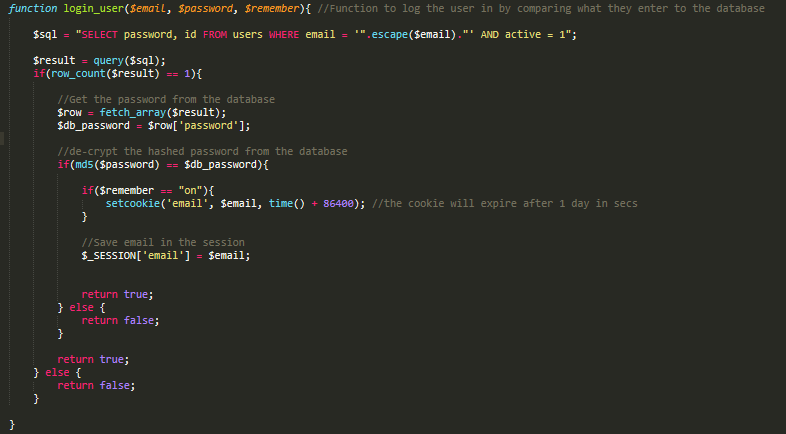
\includegraphics[width=\textwidth,height=\textheight,keepaspectratio]{img/loginUser.png}

An important part of the web application is knowing if the user is logged in. This allows the application to allow logged in users access information and functionality that is otherwise unavailable to users who are not logged in. I use a simple function to check this.

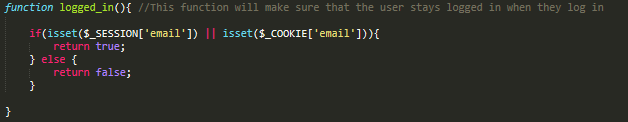
\includegraphics[width=\textwidth,height=\textheight,keepaspectratio]{img/loggedIn.png}

The final piece of the log in functionality that I wanted to get working effectively was the recover password functionality. This was a similar function to the one I used when activating a users account. Again in this function there is an email sent out containing the validation code to recover the password.

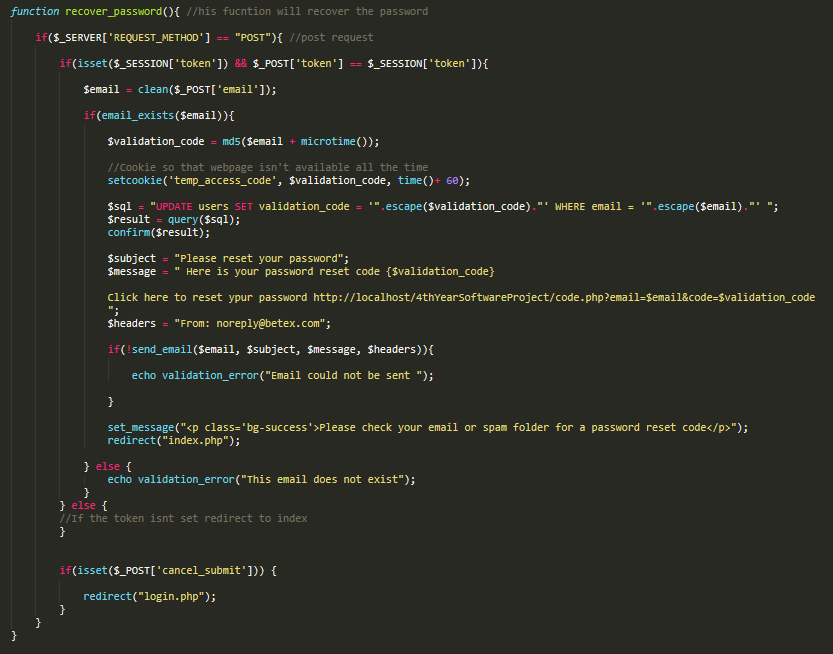
\includegraphics[width=\textwidth,height=\textheight,keepaspectratio]{img/recover.png}

Another function that I would like to highlight is the function used to place a bet. In this function I retrieve data from various tables and pass the relevant data into the table which will store the information on the stored bet. I use similar functions for when the user is laying a bet. 

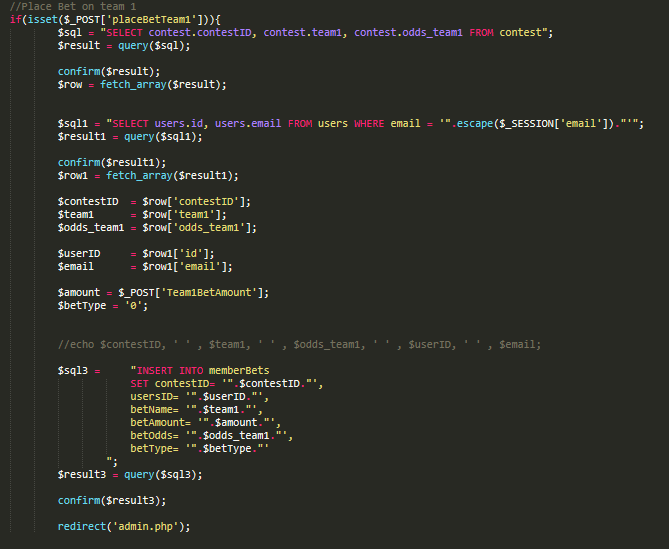
\includegraphics[width=\textwidth,height=\textheight,keepaspectratio]{img/placeBet.png}




\section{Presentation Tier}
In the presentation tier I will look at the website structure, individual pages and also deployment and hosting on a virtual machine. I will talk about design choices I made and the overall design of the application. 

\subsection{Website Structure}
In this section I will talk about the structure of my project. Below is an image of the project as it appears in Sublime Text.

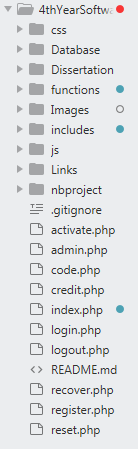
\includegraphics{img/structure.png}

In this image you can see that all of the main pages that relate directly to the website structure are in the root. From here you can then see in the folder js. In this folder you can find all the javascript related files. In here we have the jquery.js and bootstrap.js files. Above this we have the includes folder. In this folder I have placed all the php files that will be used as includes on each of the main files. An example of this is the header and footer files are in this folder as well as the nav bar file. 

Above this are images that are being used in this dissertation for example. All images on the web application are hosted online. Above the images folder we have the functions folder. Contained within this folder we have init.php which contains a function call for obstart and sessionstart which are used in the application and must be called when the application start and it also includes db.php and function.php which are two files that are also contained within the functions folder. db.php contains all of the database connection and querying functions while functions.php is a file full of all the various functions that I use throughout the application.

Above that we have the database folder in her contains a copy of the sql file used to create the database and finally we have the css folder which contains all the css files such as bootstrap.css and style.css, style.css overwrites some of bootstrap.css to make a custom theme.

\subsection{Pages}
The first picture is of what the user see's when they first visit the site, they are encouraged to sign up in order to unlock the full potential of the site.

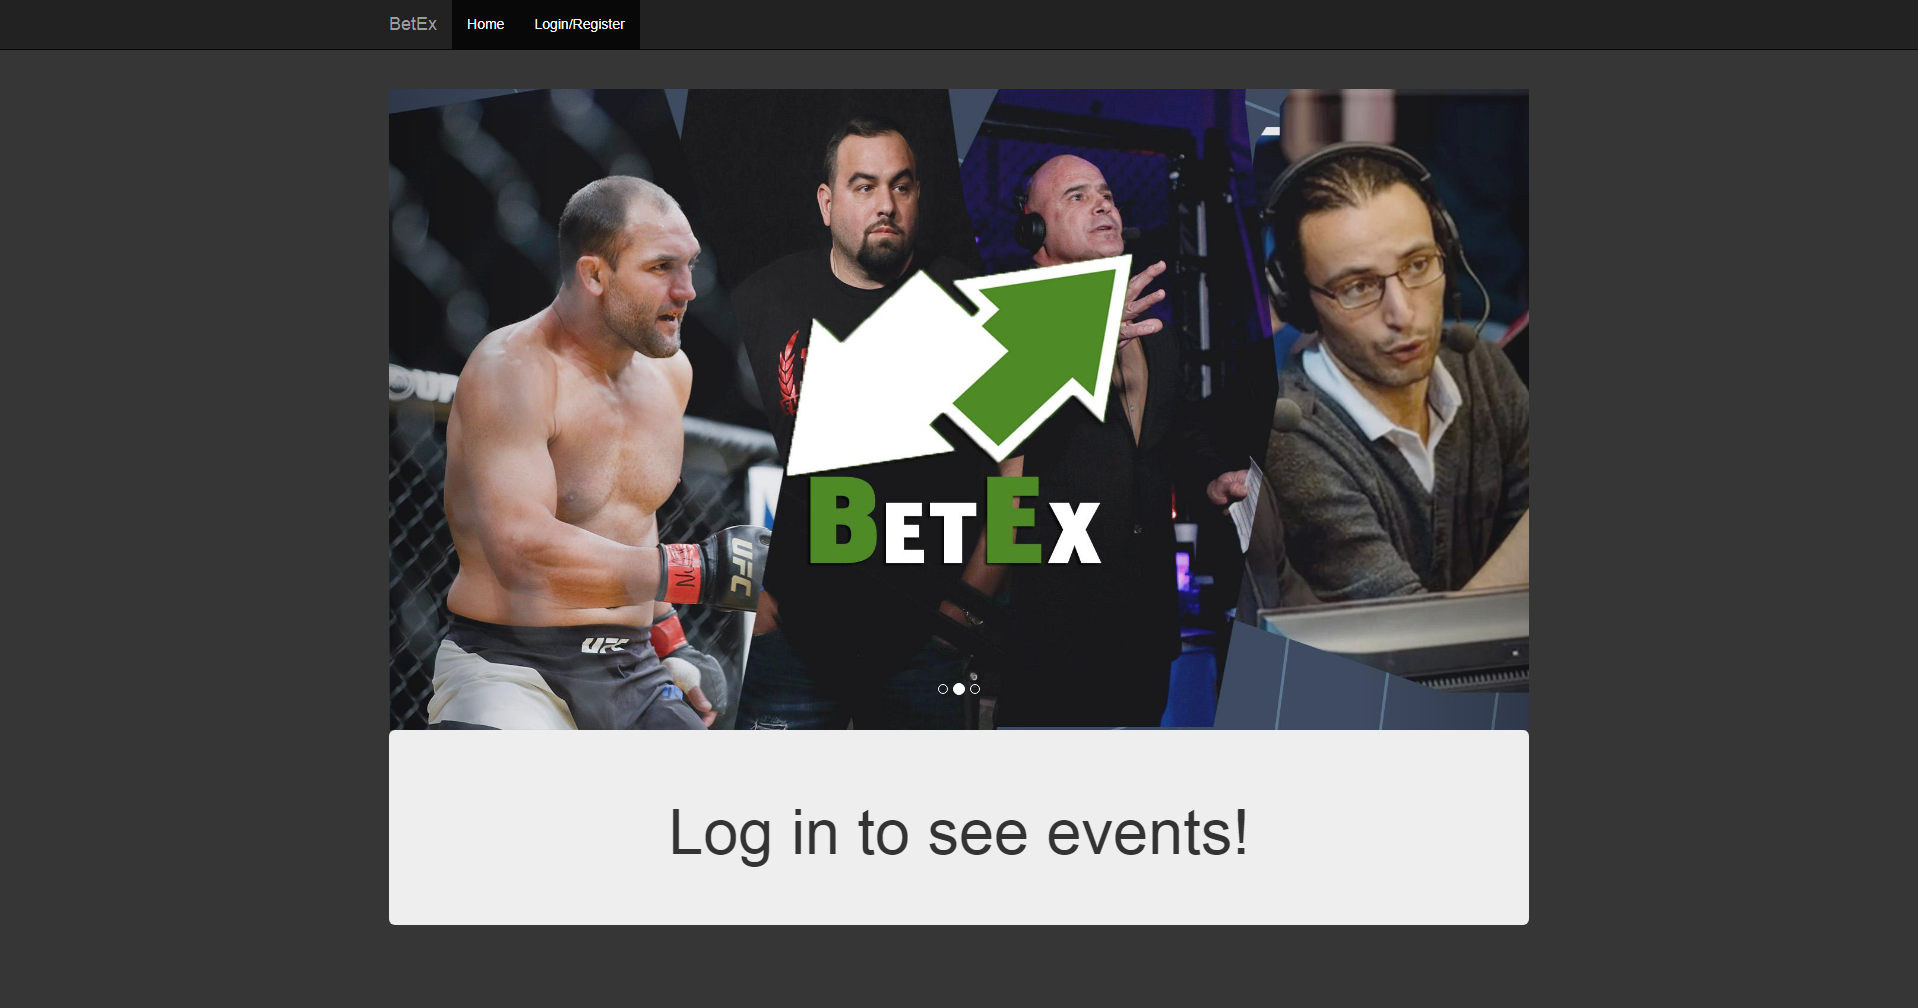
\includegraphics[width=\textwidth,height=\textheight,keepaspectratio]{img/screenshots/home.png}

From here the user is then greeted with the log in menu if the press the login/register button on the navigation menu.

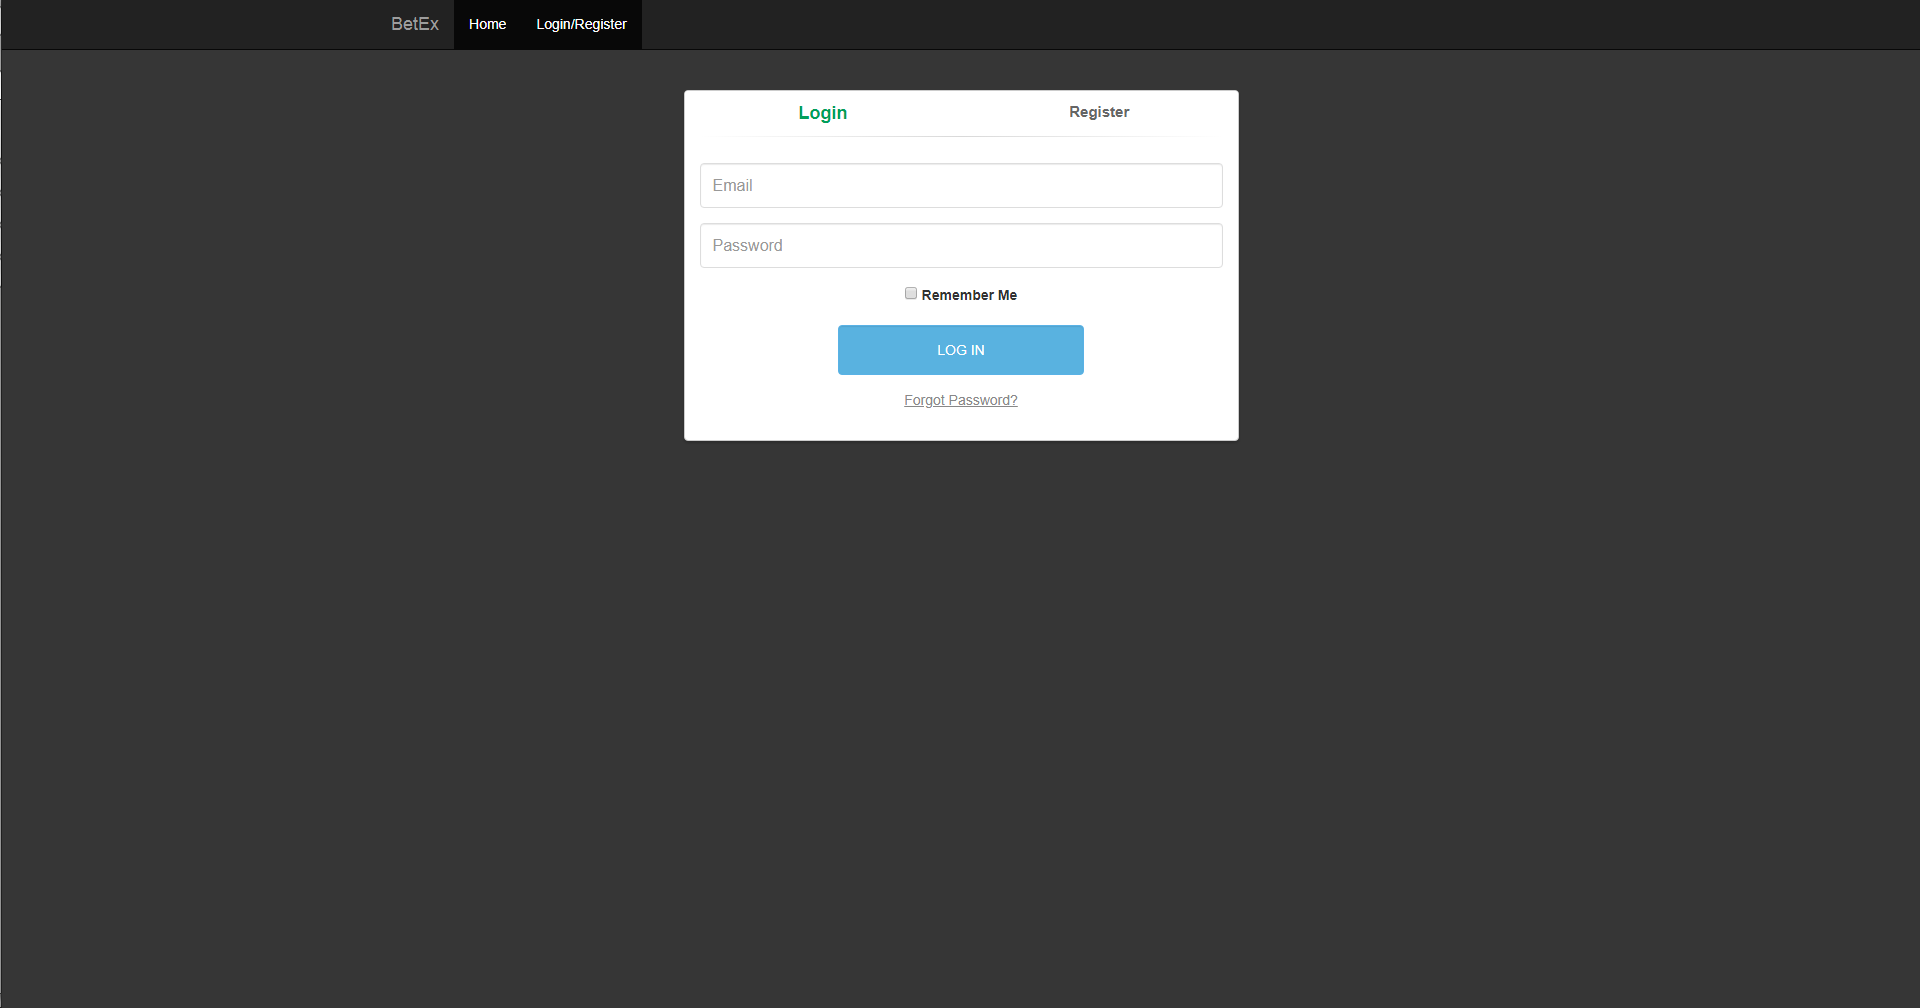
\includegraphics[width=\textwidth,height=\textheight,keepaspectratio]{img/screenshots/login.png}

On the other tab in this window is the register form it is similar to the login page.

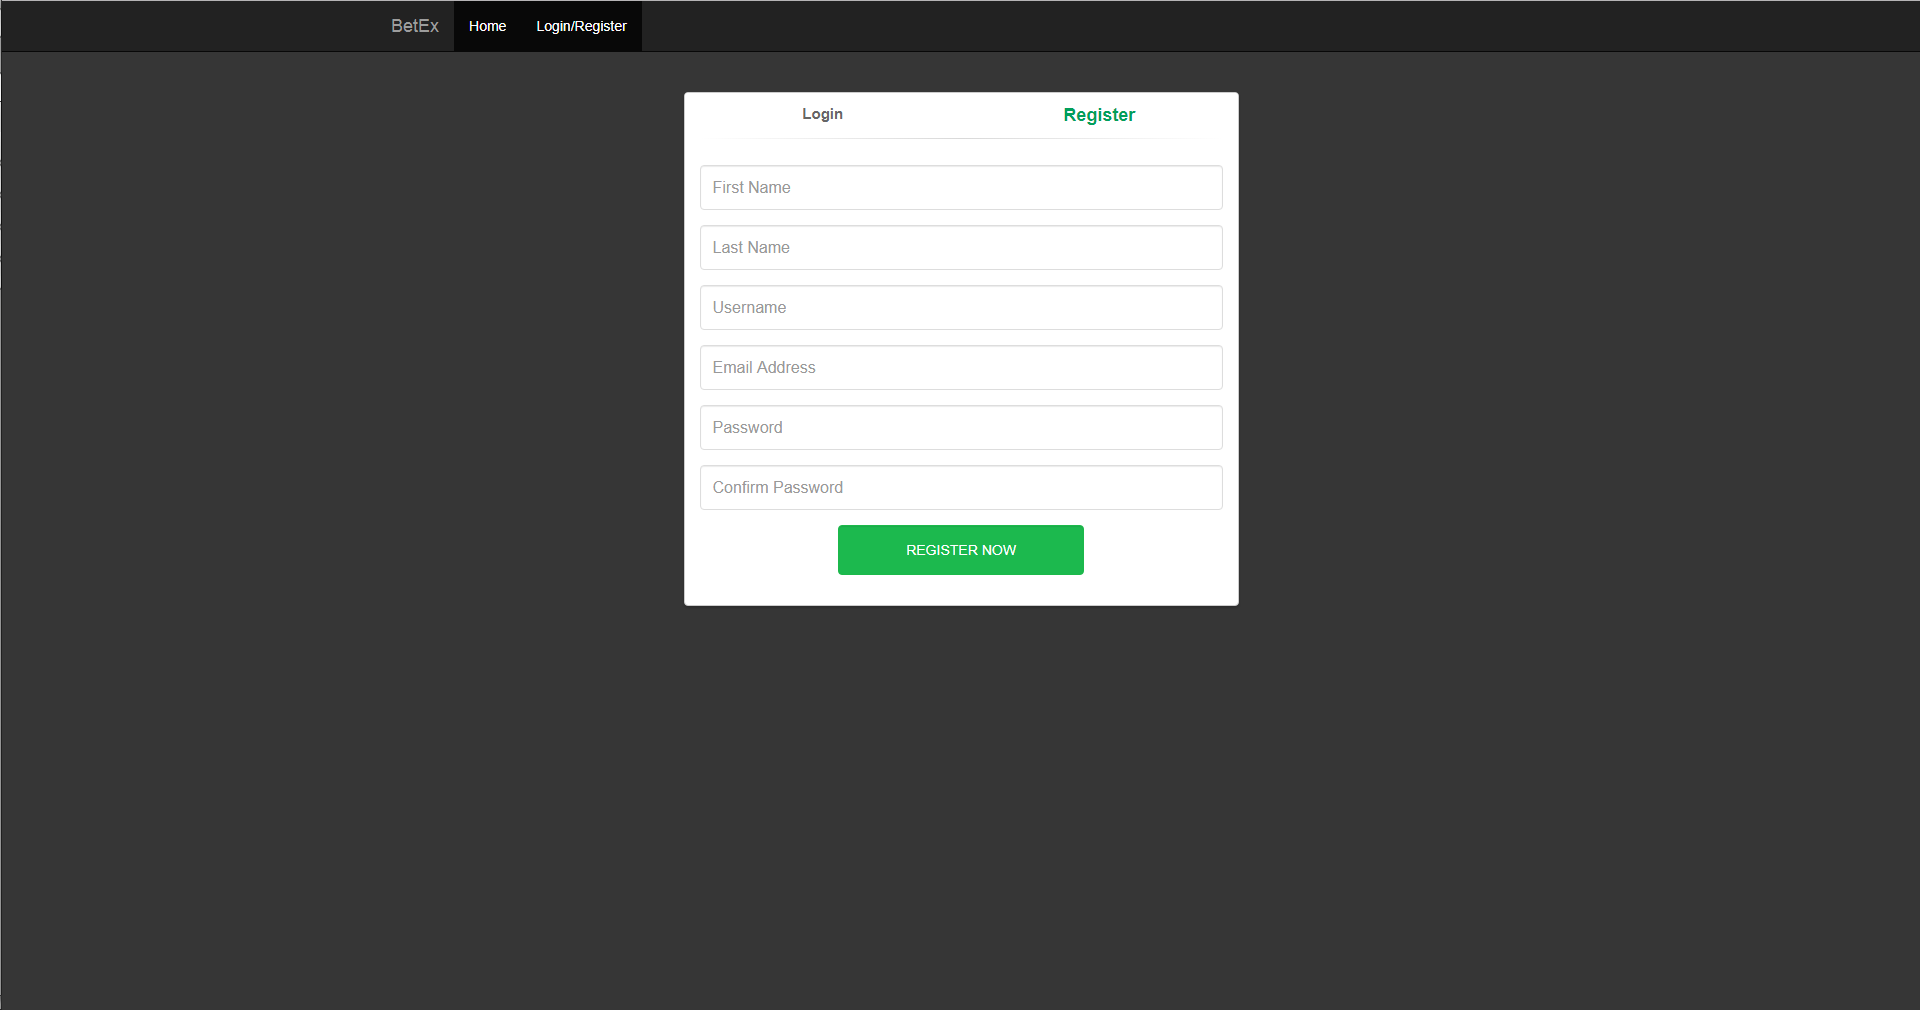
\includegraphics[width=\textwidth,height=\textheight,keepaspectratio]{img/screenshots/register.png}

You can also see the forgotten password page from here by clicking the recover password link.

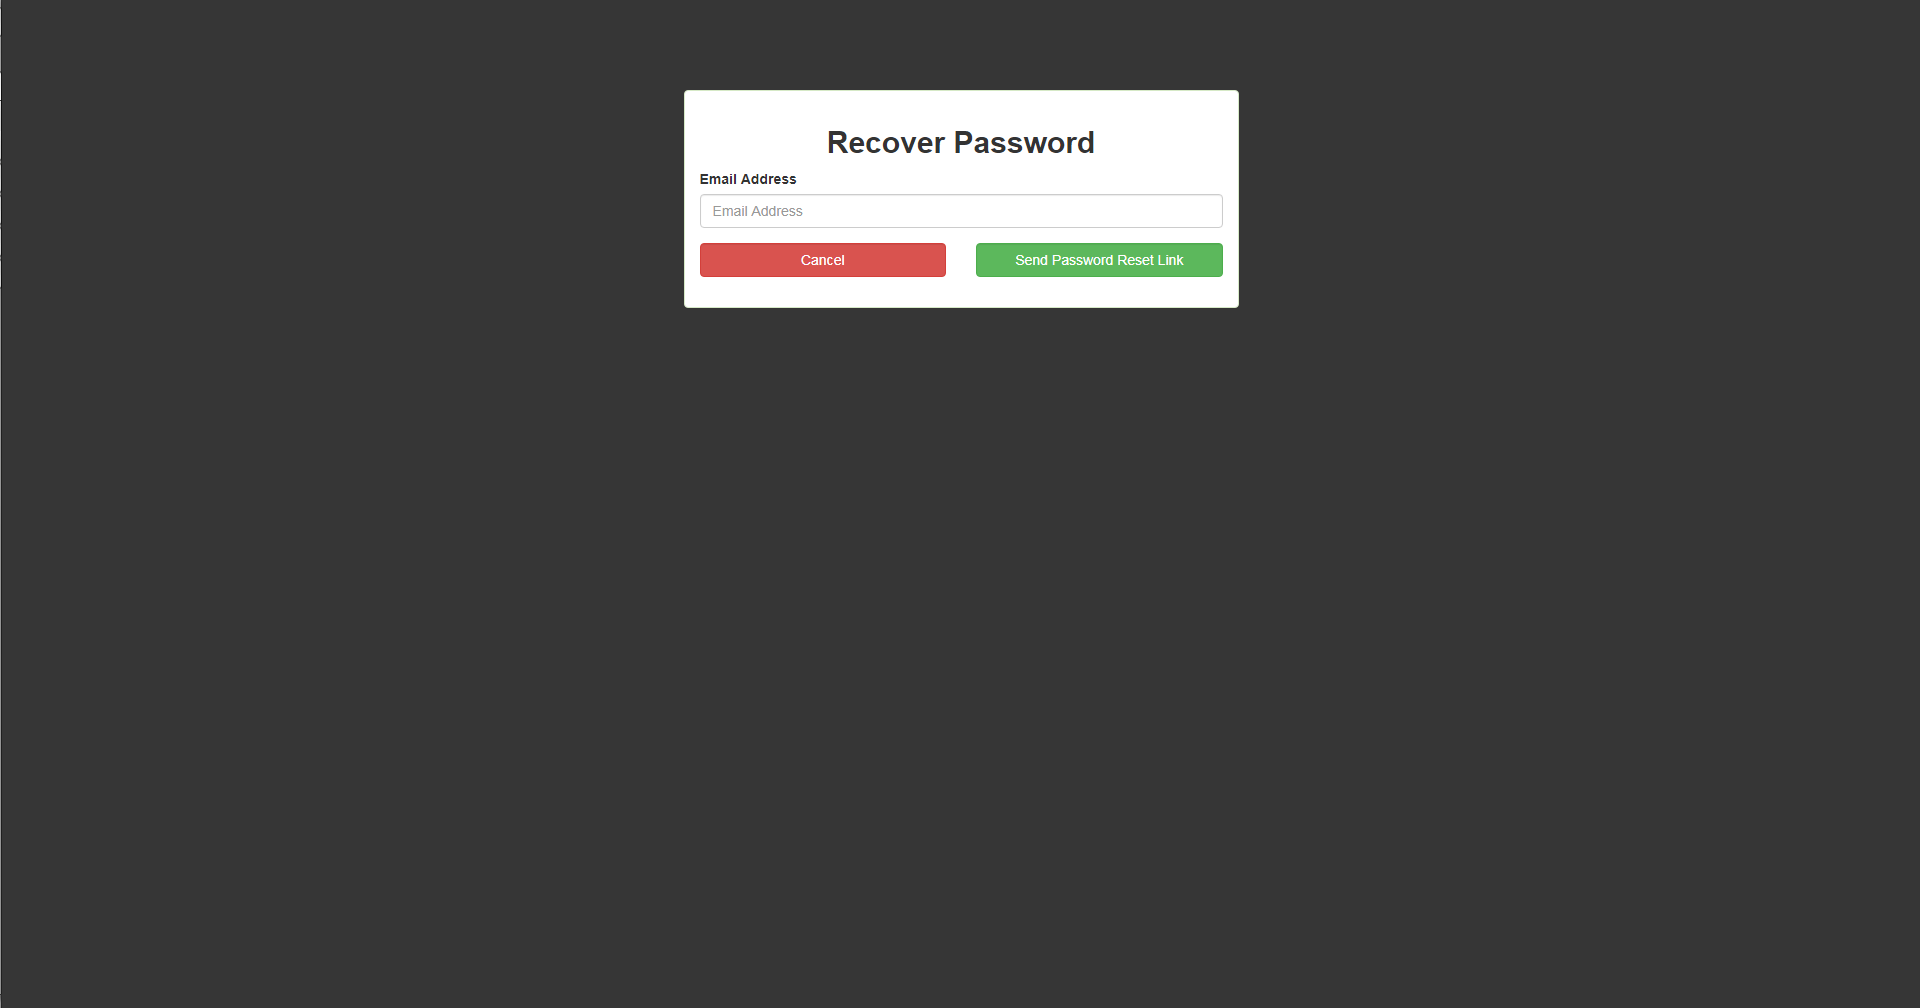
\includegraphics[width=\textwidth,height=\textheight,keepaspectratio]{img/screenshots/recover.png}

Once the user is logged in it directs the user to their profile page which will contain the history of the bets they have placed.

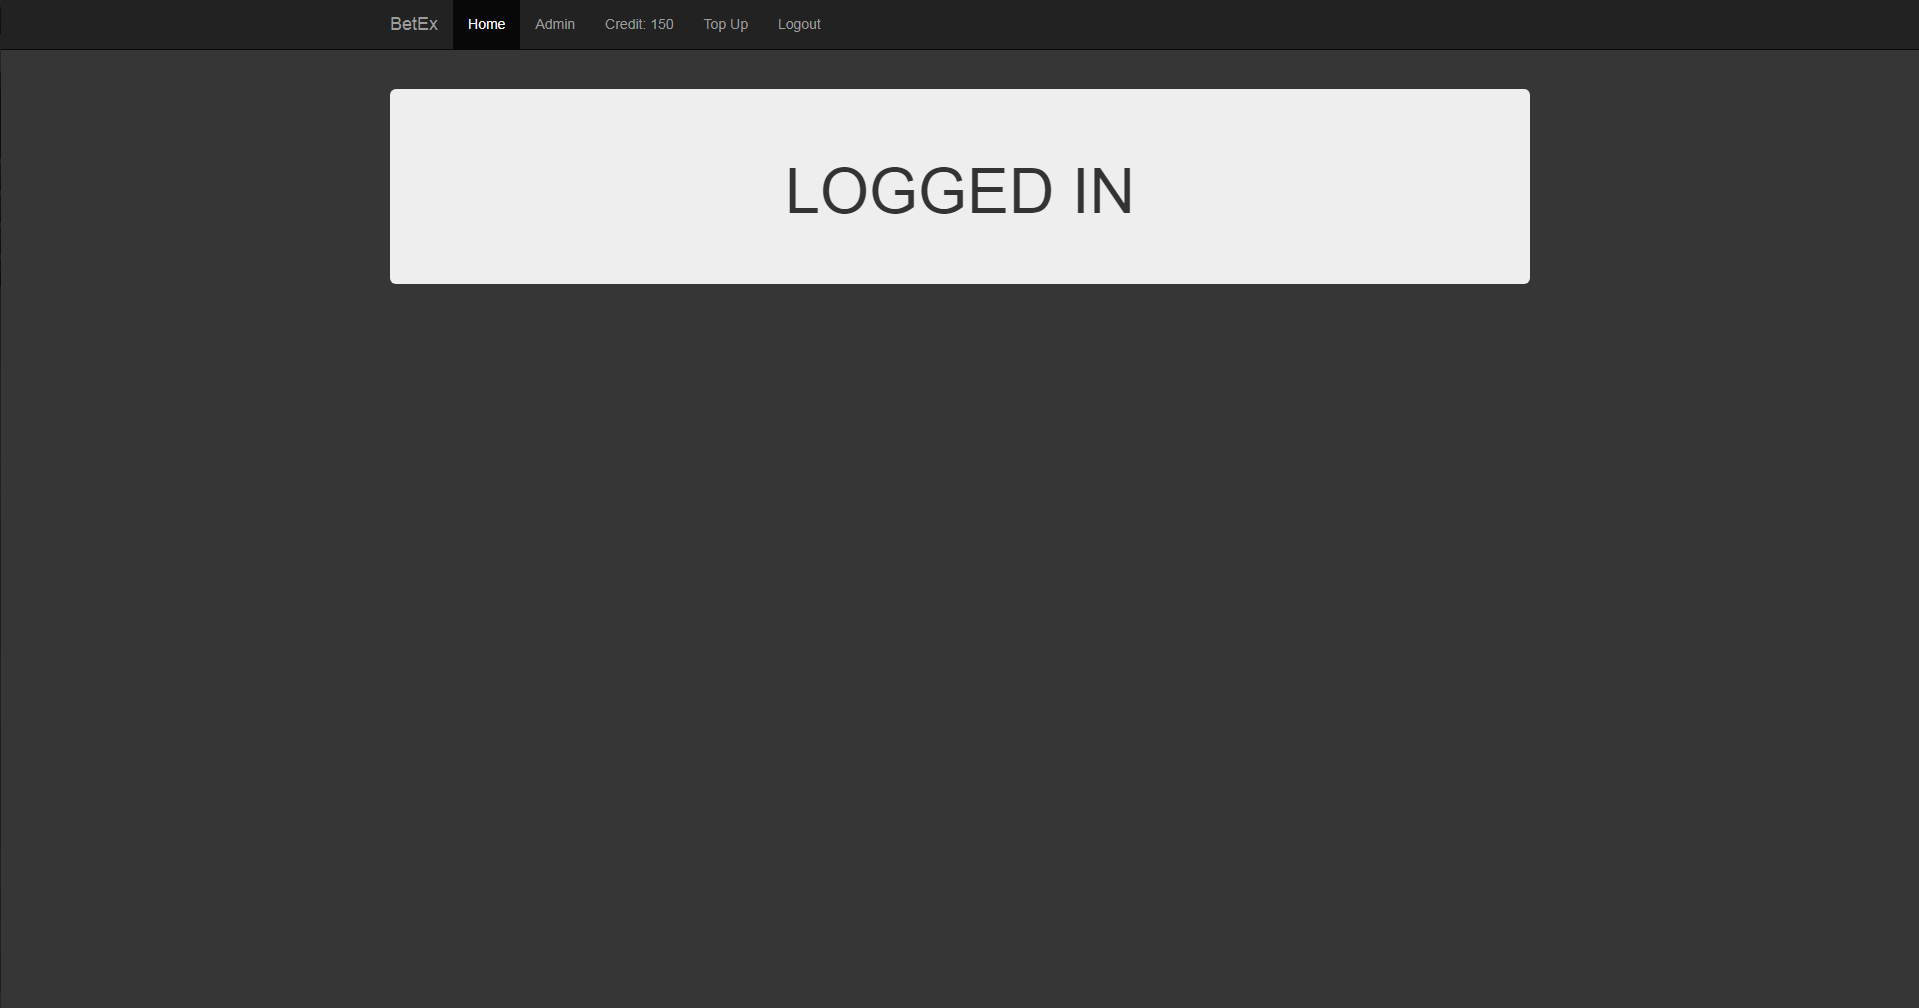
\includegraphics[width=\textwidth,height=\textheight,keepaspectratio]{img/screenshots/admin.png}

From here you can navigate back to the home page where you will now notice there are bets being displayed which you can place a bet on.

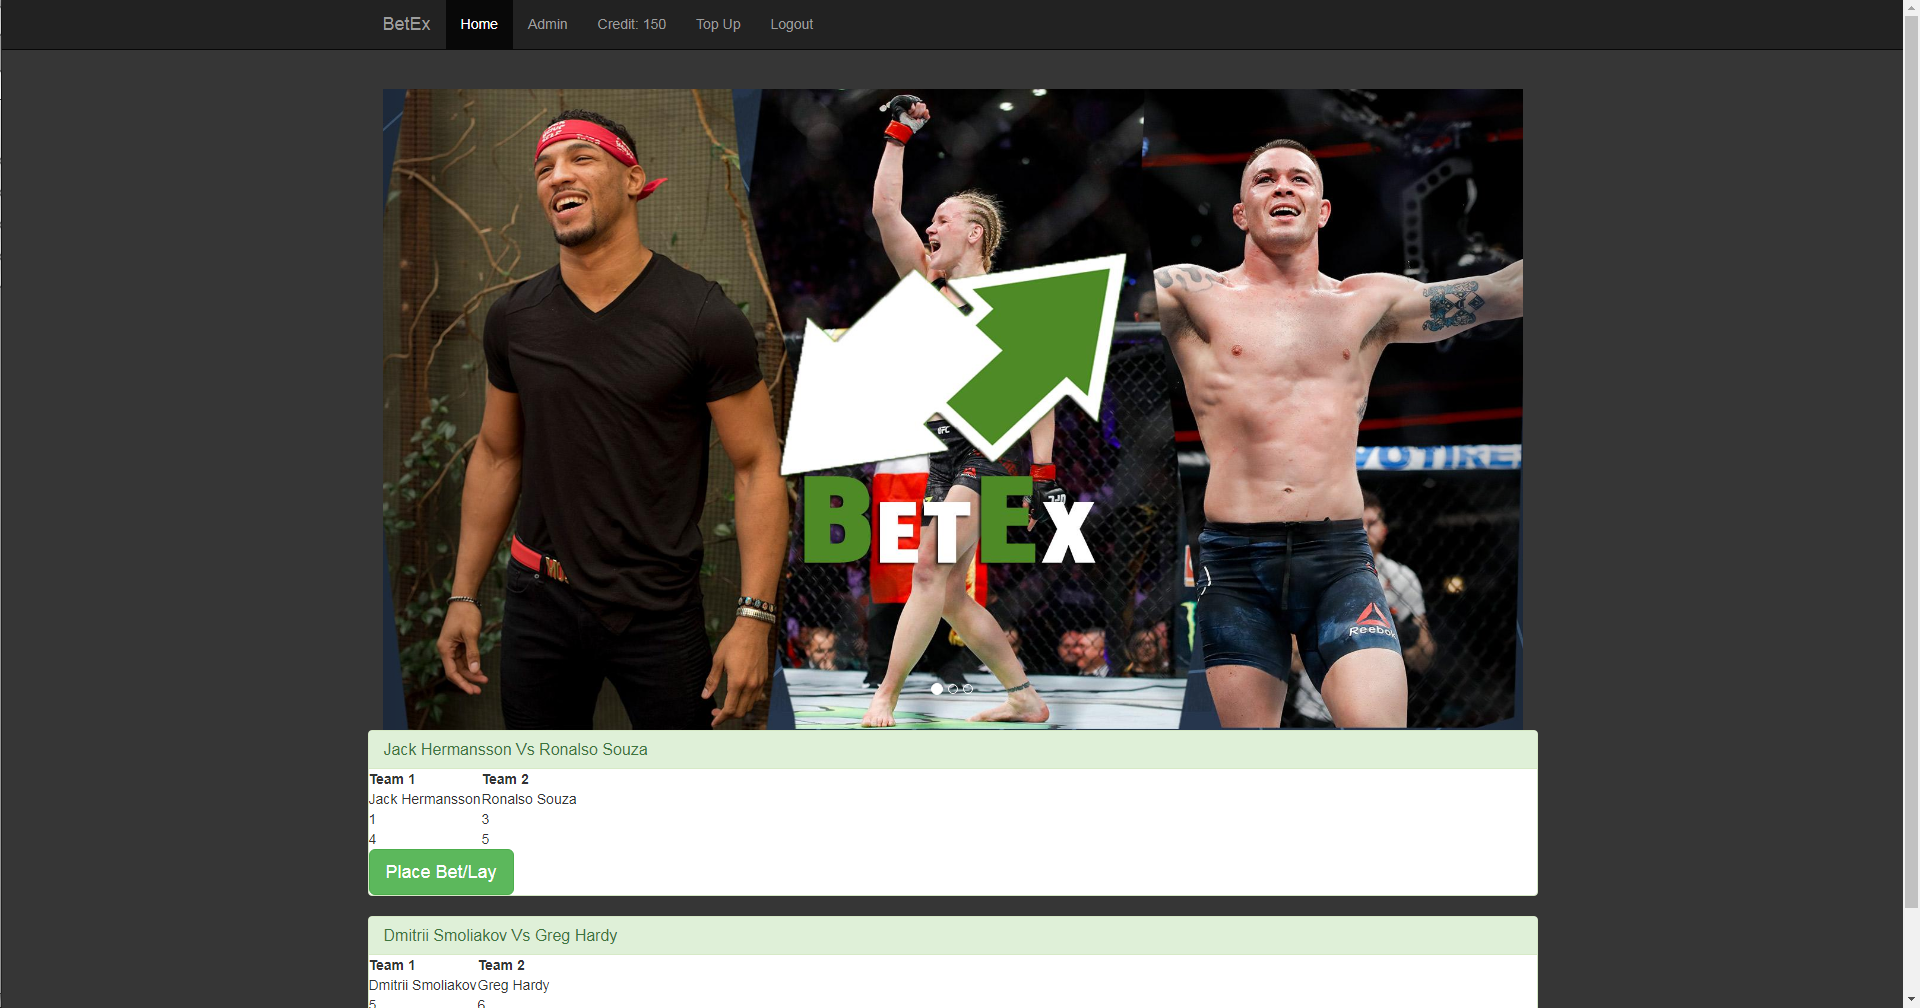
\includegraphics[width=\textwidth,height=\textheight,keepaspectratio]{img/screenshots/homeLoggedIn.png}

The two images below show the process of placing a bet.

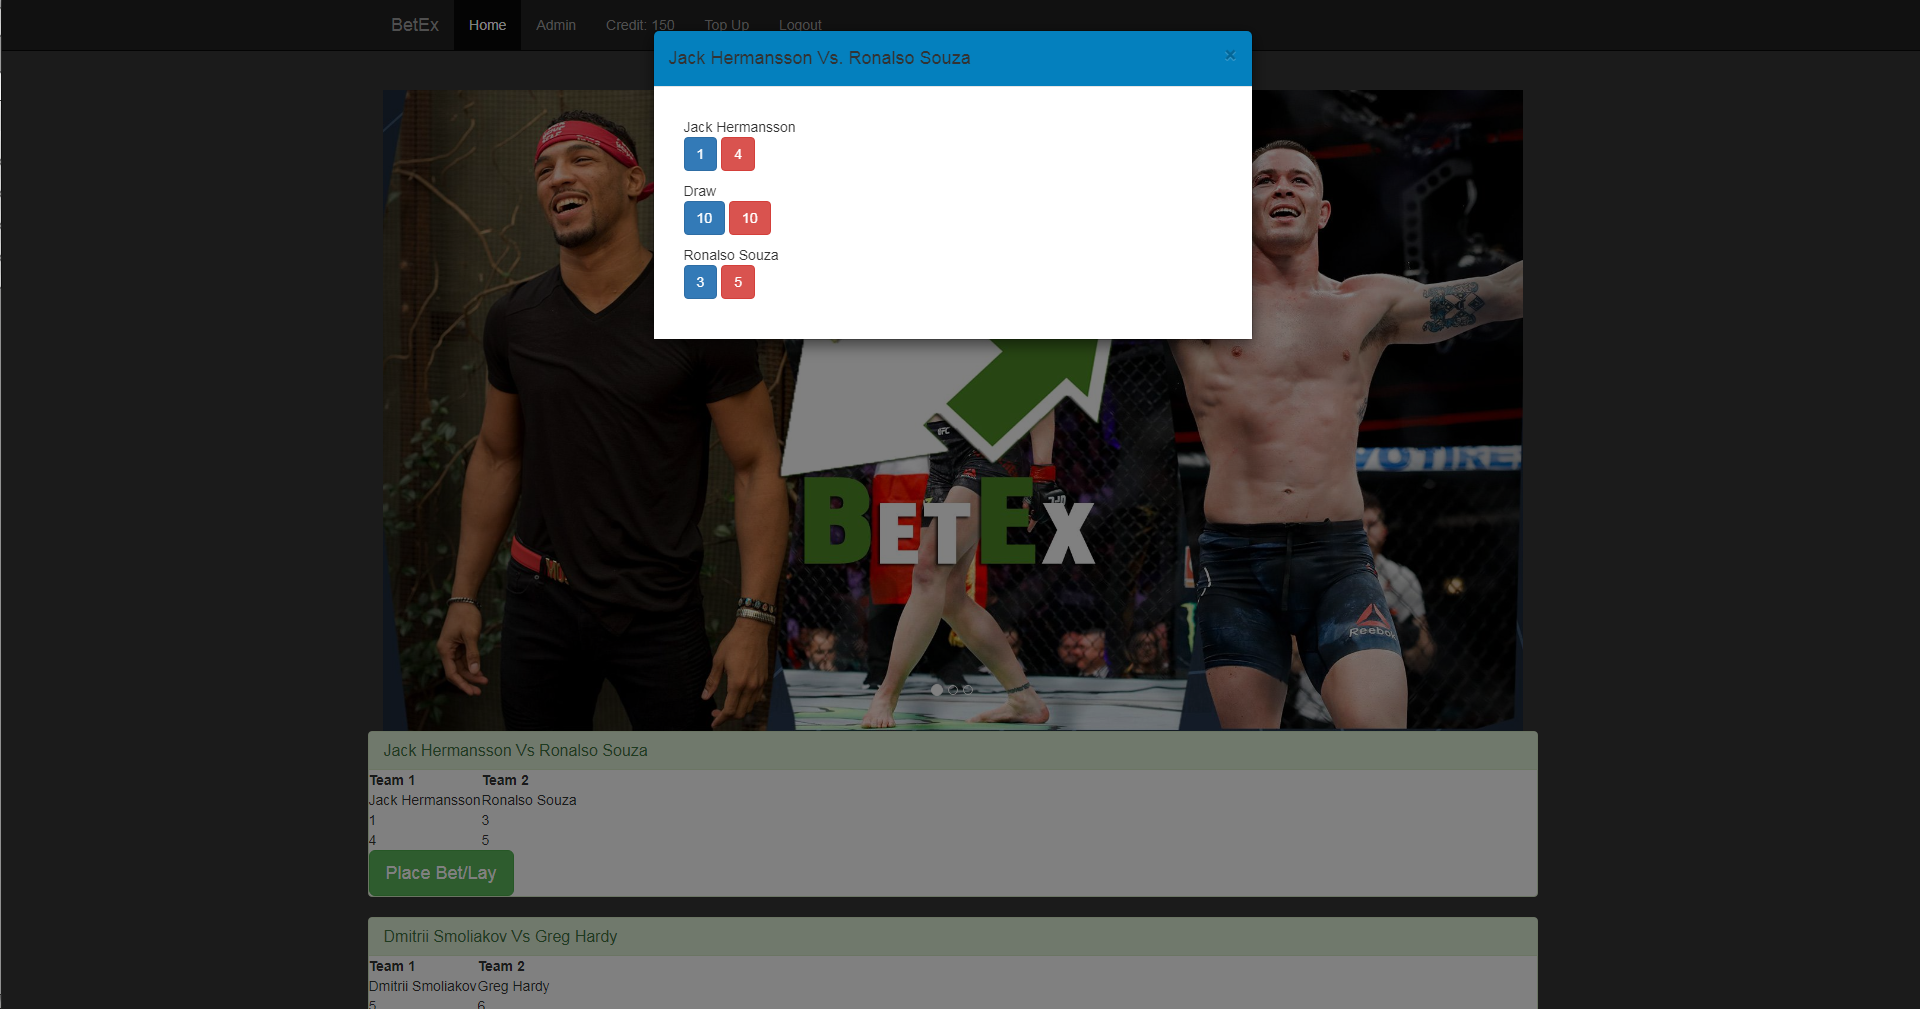
\includegraphics[width=\textwidth,height=\textheight,keepaspectratio]{img/screenshots/placeBet.png}

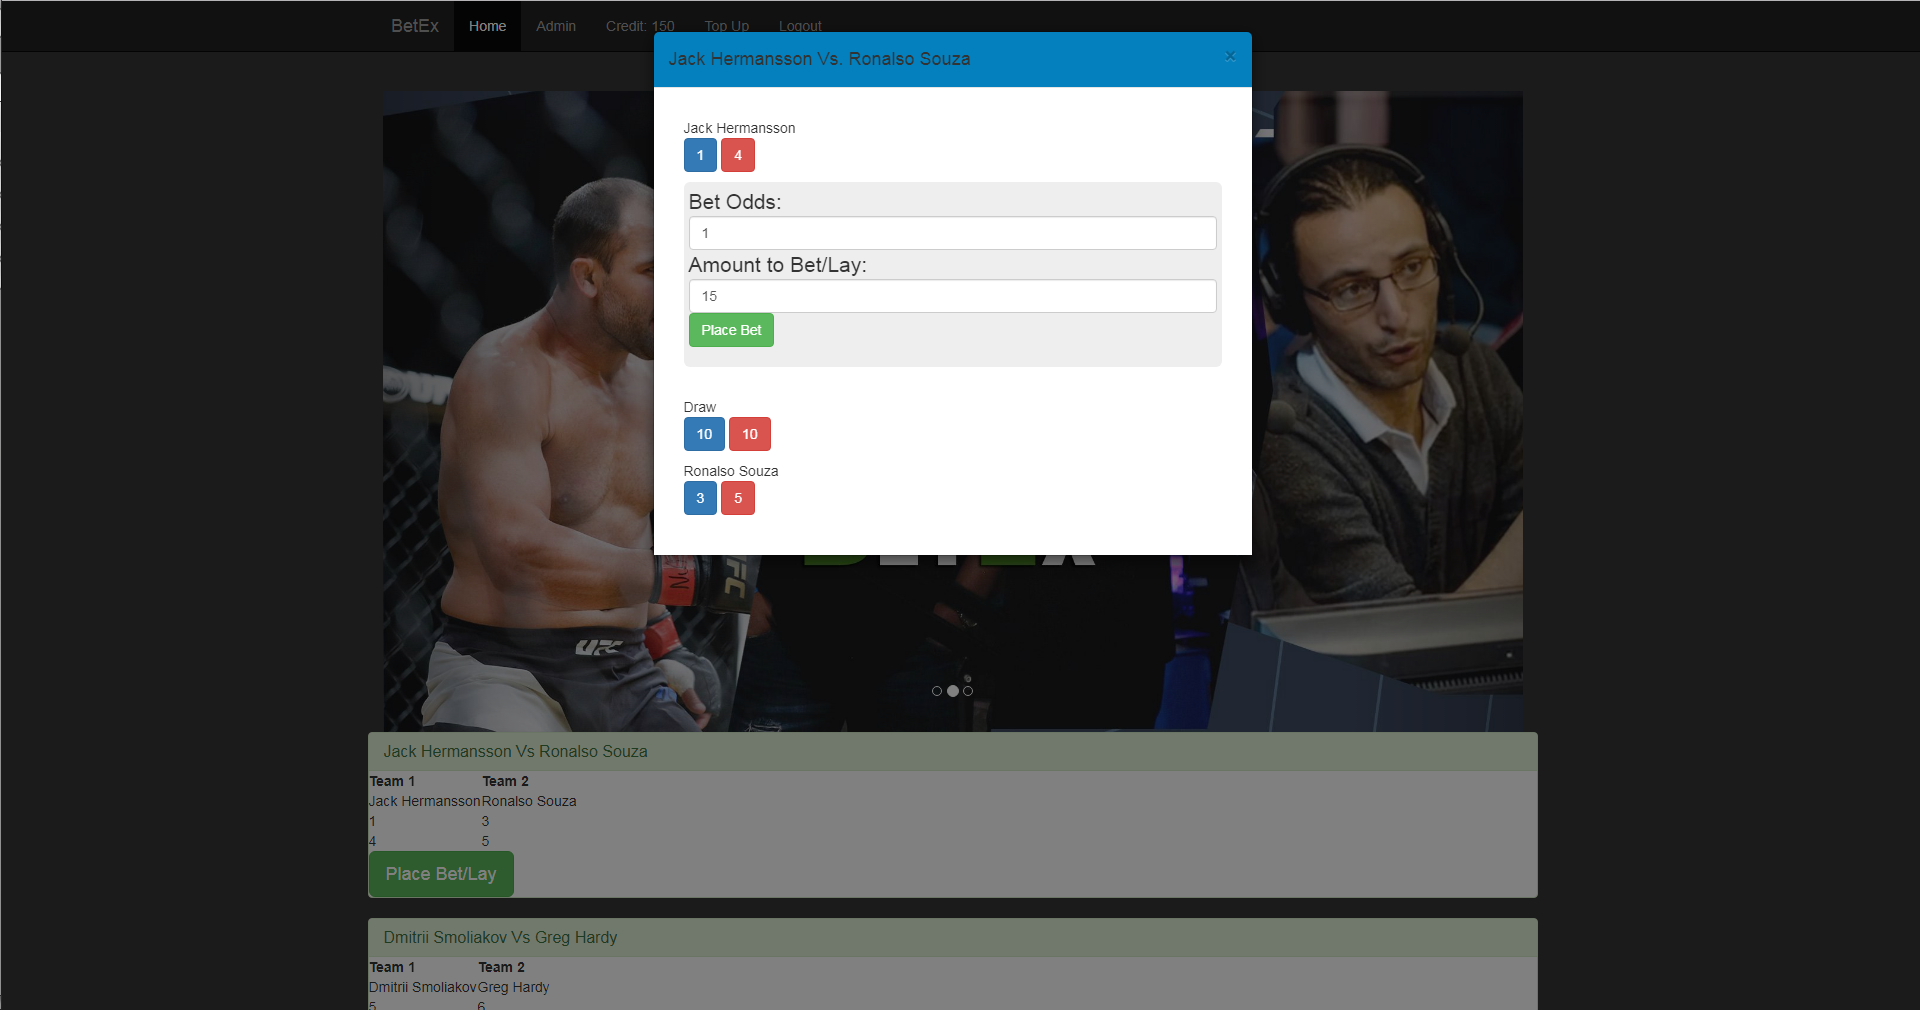
\includegraphics[width=\textwidth,height=\textheight,keepaspectratio]{img/screenshots/placingBet.png}

The final page on the site is the top up page which exists to top up the user account when they do not have enough funds.

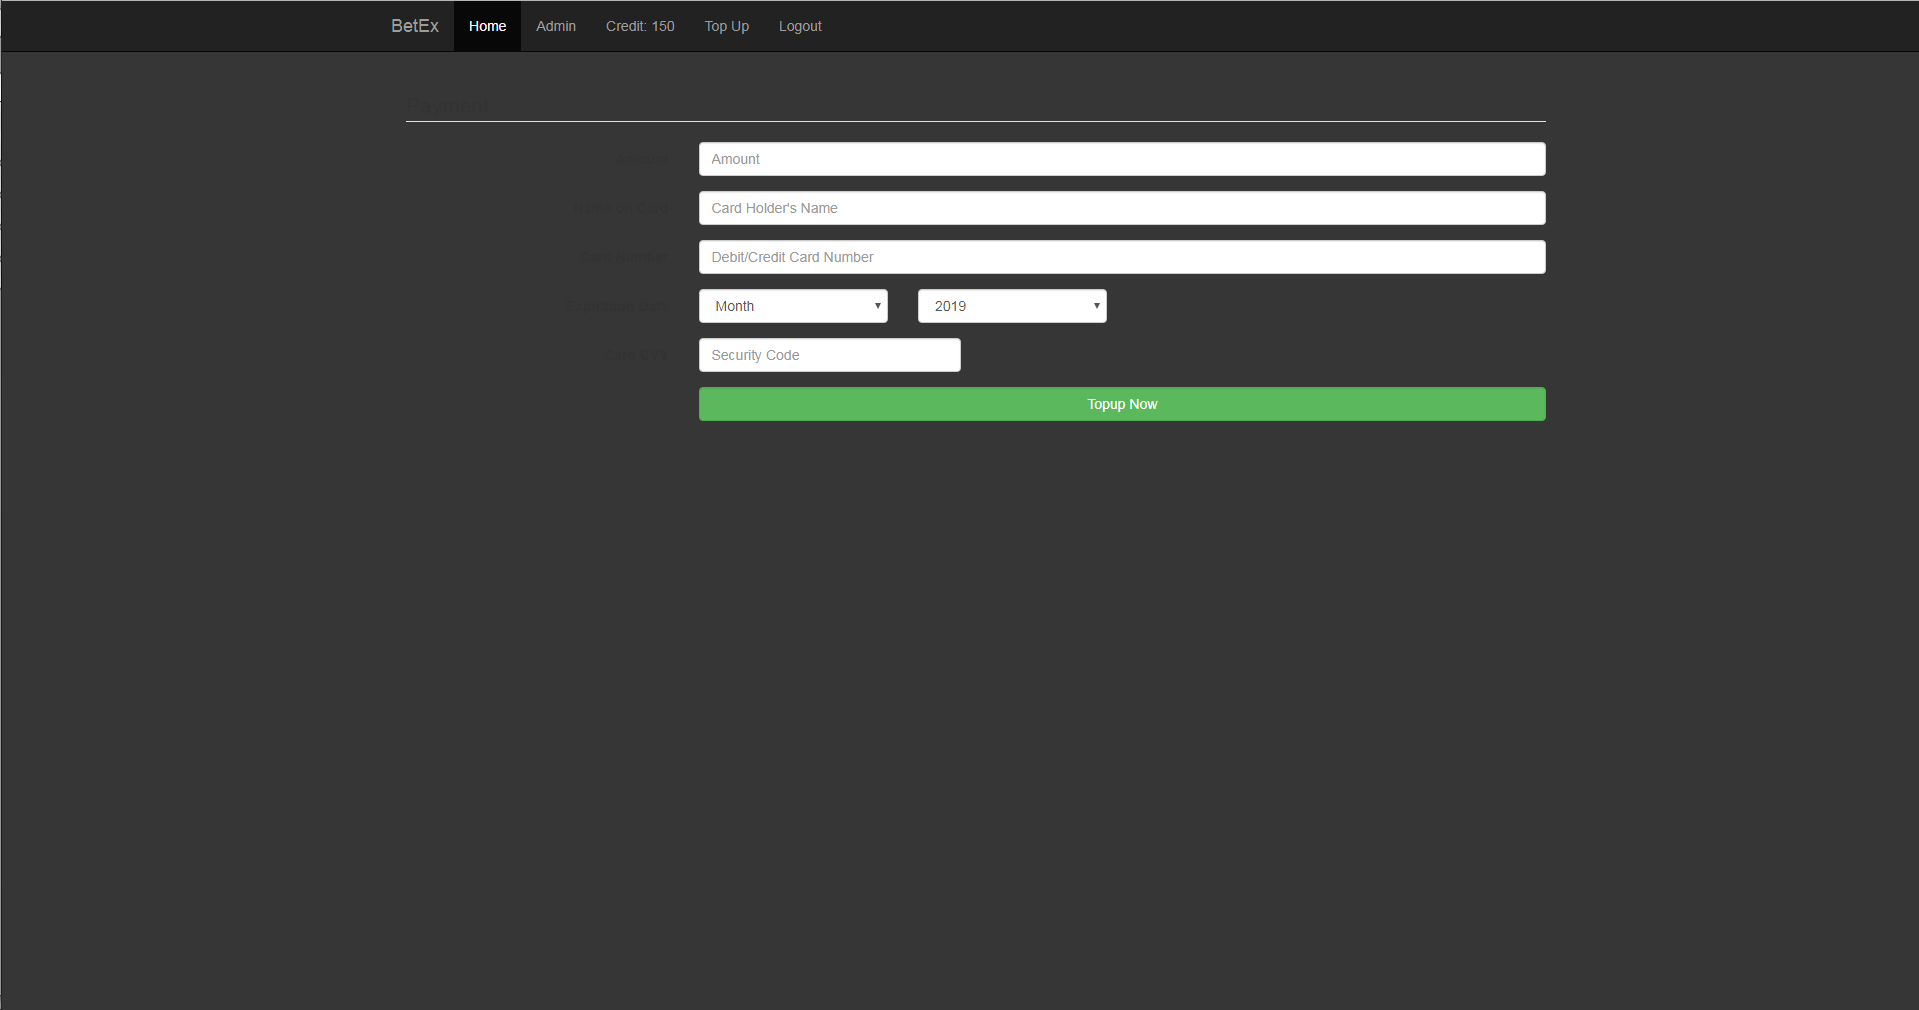
\includegraphics[width=\textwidth,height=\textheight,keepaspectratio]{img/screenshots/topup.png}

\chapter{System Evaluation}
In this chapter I will evaluate the robustness of the system, the testing and finally the limitations of the application.

\section{Robustness}
Unfortunately due to the oncoming deadline I have not been able to put the application through any real stress testing. However from regular use I have found no real bugs or errors.

\section{Testing}
\subsection{Device Testing}

\section{Limitations}
\subsection{Service Limitations}

\section{Results}

\chapter{Conclusion}
In conclusion I can say that this was most definitely the most difficult project I have attempted in my three years in Galway-Mayo Institute of Technology. The scale and complexity of the project has given me greater insight into working on bigger projects in the future. I had no major problems throughout the life cycle of the project, with time and time management being the biggest issue for myself personally. 

In the beginning I set out to create a betting exchange platform where users could place bets and lays in a user friendly environment and I can say to a certain extent I have achieved this goal.

What I have accomplished: 
\begin{itemize}

  \item Users can create an account.
  \item Users can log into their account
  \item Passwords can be reset
  \item Logged in users can view their placed bets
  \item Logged in users can view a list of bets
  \item Logged in users can place a bet or lay
  \item Logged in users can top up their account
  \item List of events is generated via a web scraping python script
  
\end{itemize}

\section{Future Development}
There are many avenues one could go in regards to future development within the app. Thoughout the development of the application to this point I have though of many features and possible things to add to the application to improve the experience. 

Once such feature might be to implement a versus league where user's can create leagues with their friends and can place bets on opposing sides with a winner take all result.

Another feature is developing the web application into a mobile application. You would then be able to put the app on the app store.

Another feature that I thought of was giving statistics to users such as betting trends displayed in graphic form.


